\documentclass{../Vorlage/sebDenCls}
\usepackage{graphicx}
\usepackage{caption}
\usepackage{subcaption}
\usepackage{listings}
\usepackage{todo}
\usepackage{longtable}
\lstset{language=C++,basicstyle=\footnotesize}
\graphicspath{ {Bilder/Doku/} }

\setcounter{section}{3}

\begin{document}
\fach{Elektronische Bildverarbeitung}
\nr{2}
\abgabe{13.06.2017}
\semester{SoSe17}
\blatt{Udo Frese}{Lukas Bertram}{Sebastian Bliefert}{Johannes Hochbein}{Pascal Pieper}


\section{}
Unsere Quest ist die automatische Erkennung von Nummernschildern an PKW und LKW. Das von uns zu entwickelnde System soll genutzt werden, um z.B. eine Schranke oder ein Tor zu öffnen. Für die Entwicklung soll ein konkreter Anwendungsfall beispielhaft genutzt werden. Dieser ist die automatische Öffnung eines Tores für bekannte Fahrzeuge in der Zufahrt zu einem Betriebsgelände. 

Der besondere Vorteil einer Identifizierung des Fahrzeugs mithilfe eines Kamerasystems ist, dass Firmenfahrzeuge, aber auch erwartete Kunden, Lieferanten und Partner (bei bekannten Kennzeichen) automatisch auf das Gelände gelangen können, da Nummernschilder einfach ein- und ausgetragen werden können. Des weiteren wäre es möglich, sich benachrichtigen zu lassen, wenn Kennzeichen „XY“ angekommen ist. So kann der jeweils verantwortliche Mitarbeiter seinen „Besuch“ in Empfang nehmen oder ähnliches. 

In unserem speziellen Fall soll die Kamera an einem Tor angebracht werden. Das Tor verfügt bereits über einen Antrieb zum Öffnen und Schließen. Unser System muss also „nur“ ein entsprechendes Signal an den vorhandenen Mechanismus senden. Eine automatische Benachrichtigung wird derzeit nicht benötigt. 

Folgende Anforderungen an das System ergeben sich aus der Anwendungssituation:
\begin{itemize}
\item Zu erkennende Kennzeichen: europäische Standardkennzeichen
\item Einsatzort des Systems: in Grundstückszufahrten
\item Abstand Fahrzeug zur Kamera: 1-2m
\item Montagehöhe der Kamera: 0,5-1m
\item Leichte Winkeländerungen des Fahrzeugs dürfen nicht zu Fehlerkennungen führen
\item Korrekte Funktion zu allen Tageszeiten
\end{itemize}	

\newpage
\section{}

Um eine Grundlage für die Entwicklung der Bildverarbeitungssoftware zu schaffen, wurden Bildern von 3 unterschiedlichen Fahrzeugen aufgenommen. Folgende Anordnung wurde dazu verwendet:

\begin{figure}[htp]

	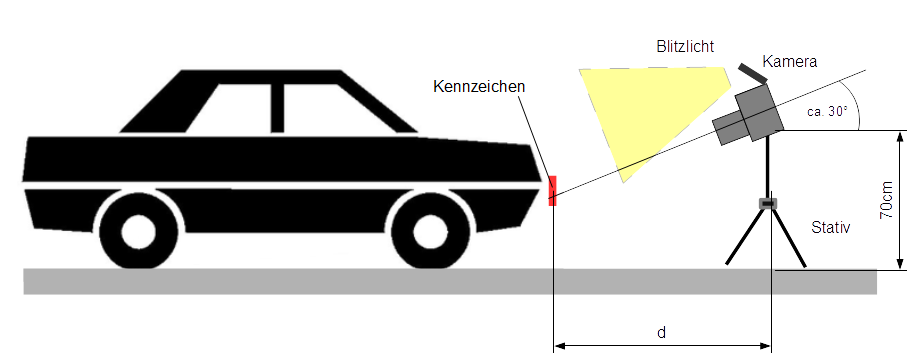
\includegraphics[width=.9\textwidth]{Skizze_Aufg_5_seite} 
	\caption{Seitenansicht \label{seitenansicht}}
\end{figure}

\begin{figure}[htp]
		\centering 	
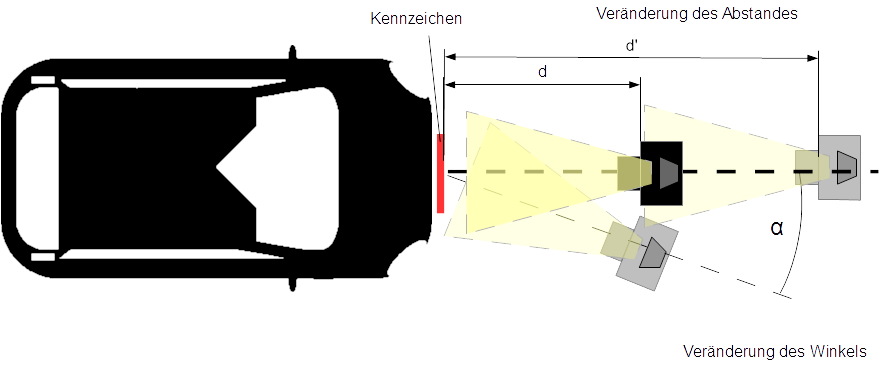
\includegraphics[width=.9\textwidth]{Skizze_Aufg_5_oben} 
\caption{Draufsicht\label{draufsicht}}
\end{figure}

Der Abstand \emph{d} wurde für jedes Fahrzeug im Intervall von 1m - 2m schrittweise um 20cm erhöht. Dies wurde für Winkelwerte $\alpha = -20^\circ,-10^\circ,+10^\circ,+20^\circ$ wiederholt.


Die Bilder wurden aufgenommen mit einer Canon 750D Spiegelreflexkamera und folgenden Aufnahmeparametern:

\begin{center}
\begin{tabular} {| l | r |}
	\hline
Brennweite: & 24mm \\ \hline
Blendenzahl: & 22 \\\hline
Belichtungszeit: & 1/200s \\\hline
ISO: & 400 \\\hline
Interner Blitz: & aktiviert \\\hline
\end{tabular}
\end{center}


Der Fokus wurde manuell bei einer Entfernung von einem Meter eingestellt und danach nicht weiter verändert. 

\begin{figure}[htp]
	\centering 	
	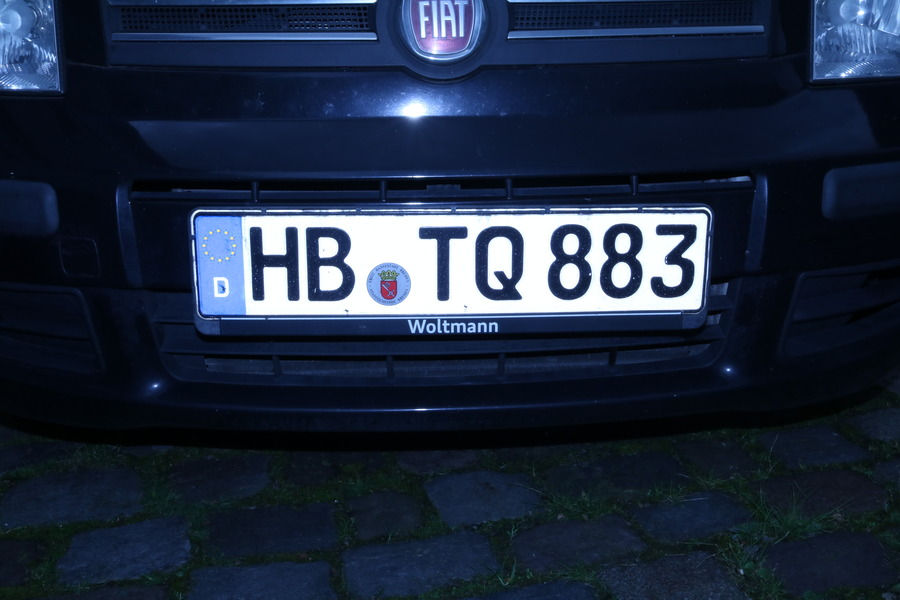
\includegraphics[width=.9\textwidth]{beispielbild} 
	\caption{Beispielbild: Abstand $d=1m$, Winkel $\alpha = 0^\circ$ \label{beispiel}}
\end{figure}

\begin{figure}[htp]
	\centering 	
	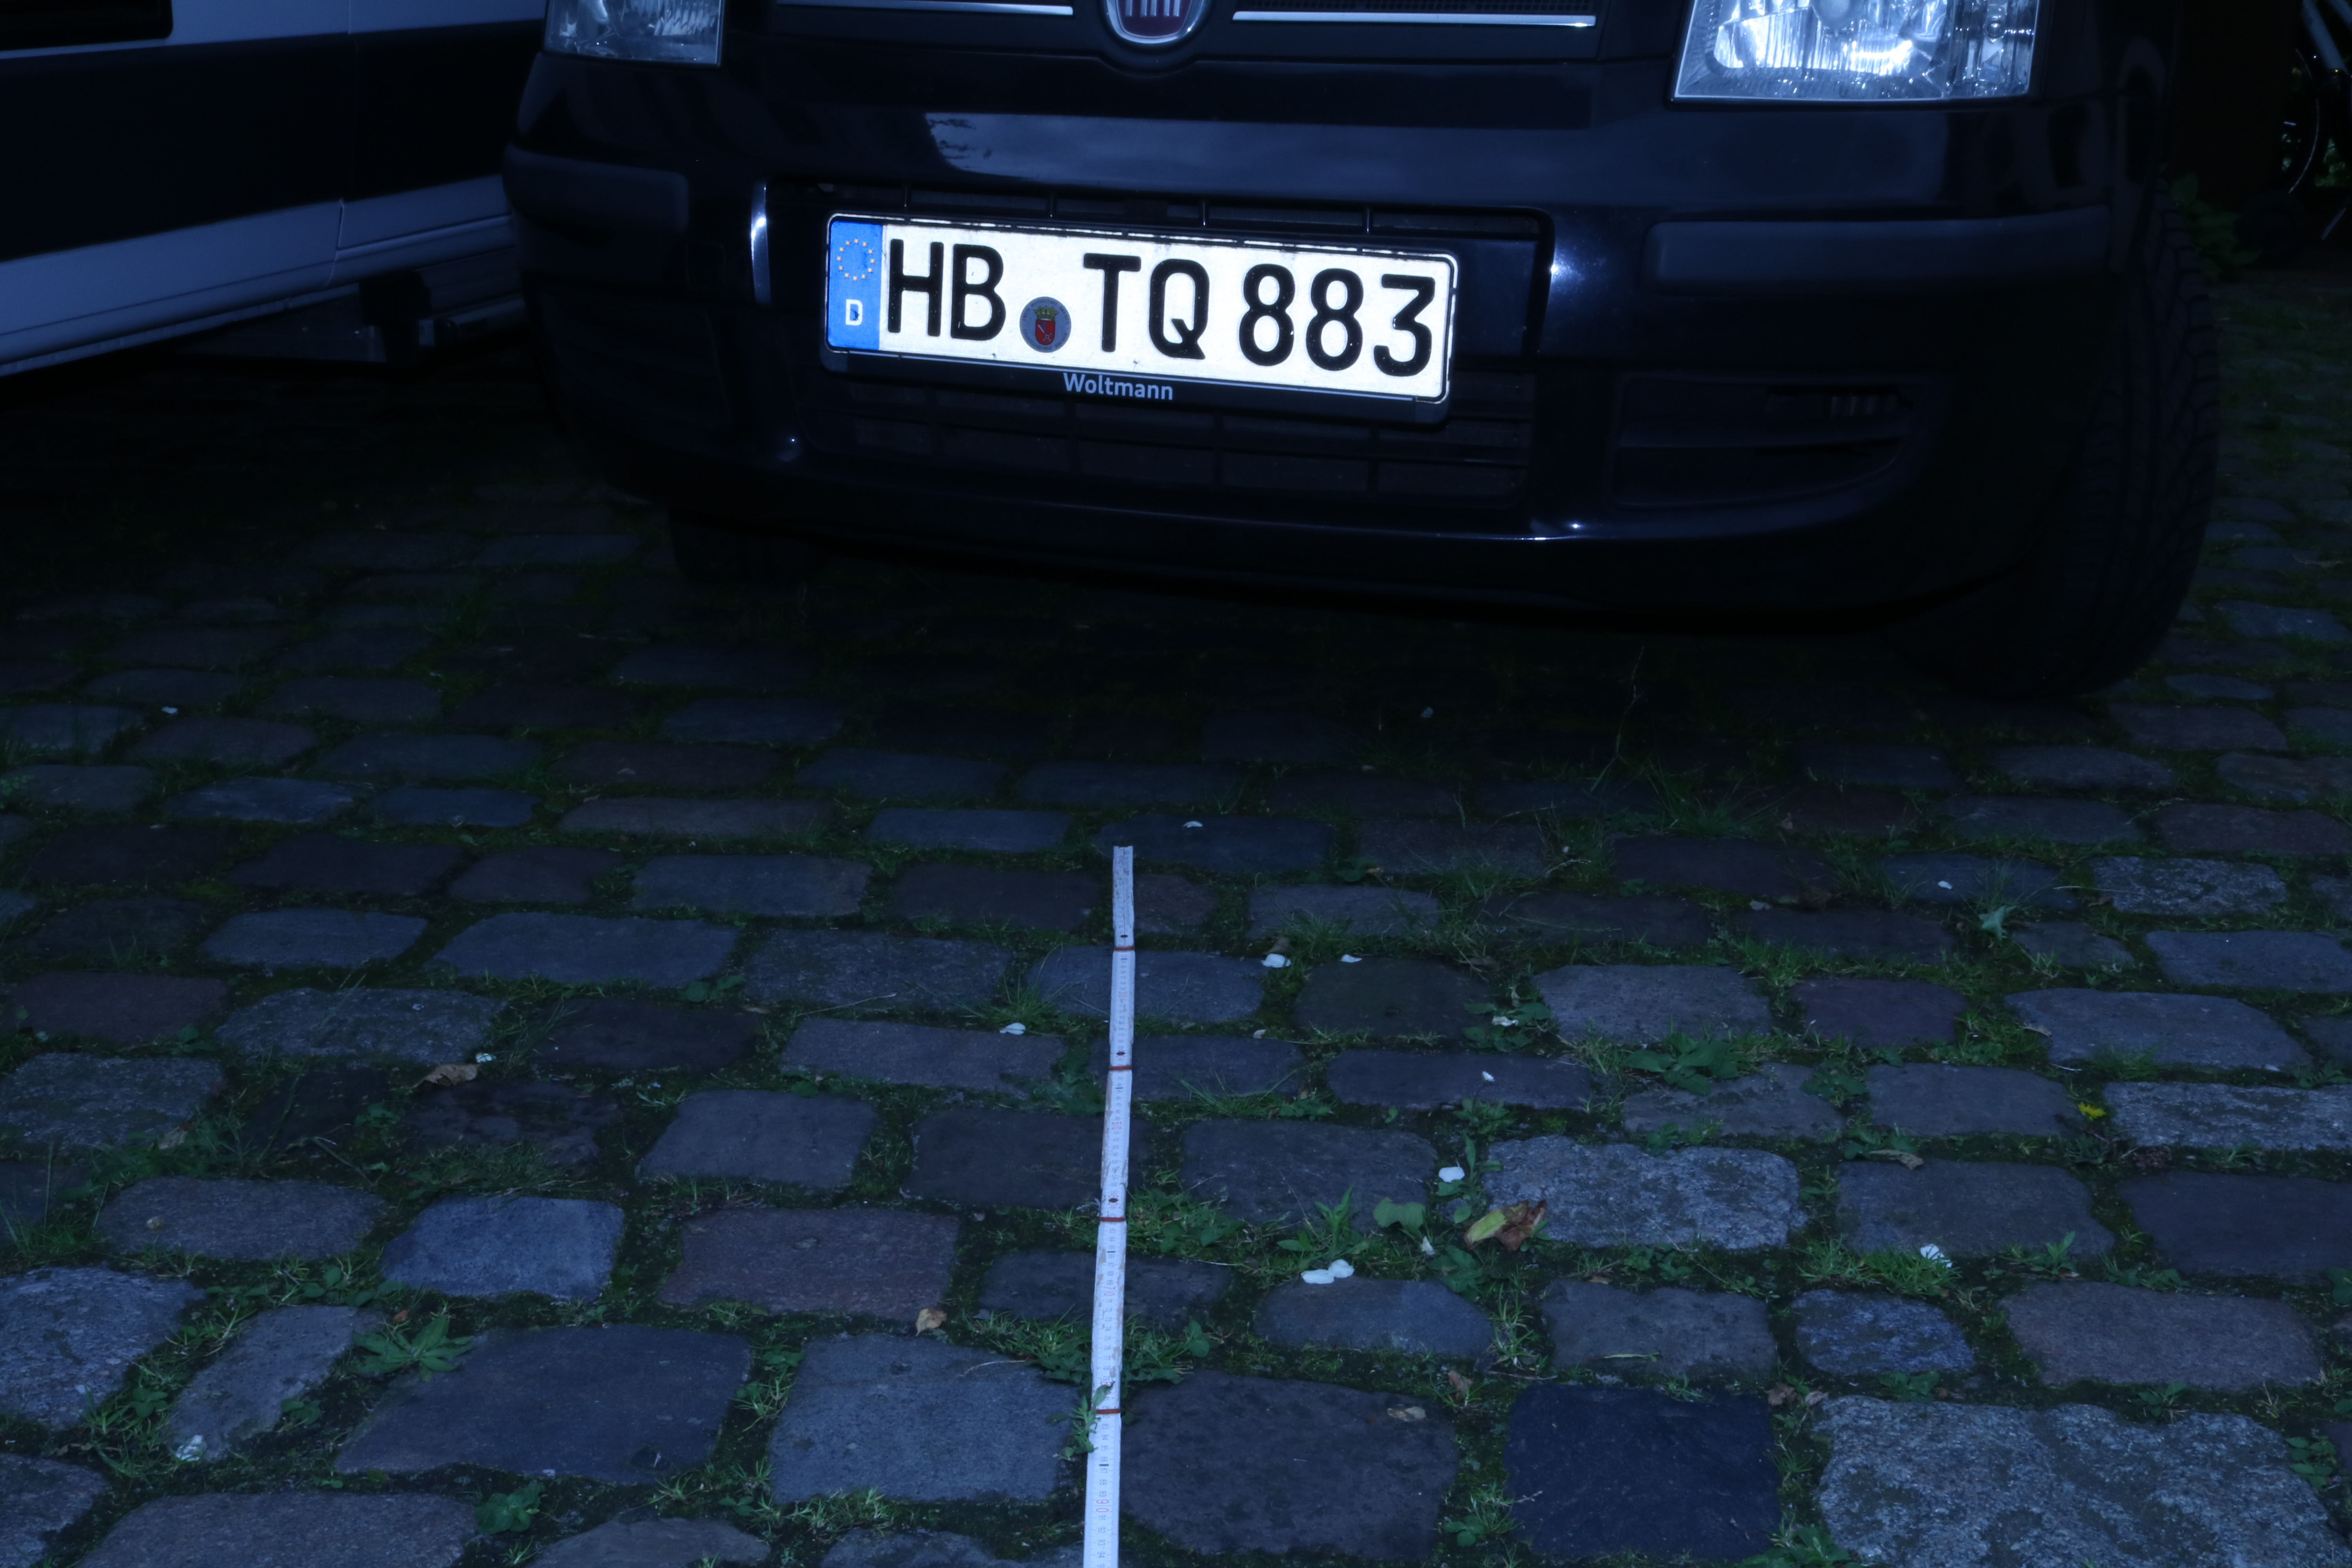
\includegraphics[width=.9\textwidth]{beispielbild2} 
	\caption{Beispielbild: Abstand $d=2m$, Winkel $\alpha = 20^\circ$ \label{beispiel2}}
\end{figure}

\section{}

Der Hardwareaufbau unseres Lösungsansatzes ist grundlegend bereits durch die Aufgabenstellung definiert.\\
Die Kamera wird in einer Höhe von 50-100cm montiert, zum Beispiel an einem Tor. Dabei ist sie aus Datenschutzgründen leicht nach unten gerichtet, sodass Fußgänger deutlich unterhalb des Kopfes abgeschnitten werden. Aufgrund des geringen Abstandes zum Fahrzeug sollte ein Weitwinkelobjektiv (bspw. 24mm) verwendet werden. Um ein ausreichend scharfes Bild zu gewährleisten, sollte mit möglichst kleiner Blende fotografiert werden, sodass eine ausreichende Tiefenschärfe gegeben ist. \\
\\
Zur Verringerung des Einflusses von Umgebungslicht verfügt das System über eine eigene Lichtquelle, realisiert bspw. durch ein koaxiales Ringlicht. Bei ausreichender Beleuchtungsstärke kann so in Kombination mit einer möglichst kleinen Blende und kurzer Belichtungszeit der Anteil des Umgebungslichtes bei der Belichtung reduziert werden.\\
Um den Einfluss von Fremdlicht noch weiter zu reduzieren und den störenden Einfluss der Beleuchtung auf die Verkehrsteilnehmer zu verringern, könnte die Verwendung einer Infrarotbeleuchtung in Kombination mit einem entsprechenden Bandpassfilter in Betracht gezogen werden. Im Kontext des Übungsprojektes wird vom Einsatz dieser Komponenten aber aufgrund von Materiallieferzeiten abgesehen.
\\
Die Anordnung der Systemkomponenten hat den Vorteil, dass ankommende Fahrzeuge bereits in einer gewissen Distanz gesehen werden, so kann das Tor bereits geöffnet werden und es ergeben sich keine Wartezeiten. Sollten Schwierigkeiten bei der Erkennung entstehen, würde das Fahrzeug immer näher kommen und das Kennzeichen immer besser zu erkennen sein, sodass es bei Schwierigkeiten eventuell erst etwas später zu einer Erkennung kommt dies aber hauptsächlich einen Einfluss auf den „Komfort“ des Systems hat und nicht zu einen tatsächlichen Ausfall führt.

Aus Gründen der Energiesparsamkeit und des Datneschutzes verwenden wir einen Trigger (zum Beispiel einen Ultraschalldistanzsensor), der im Distanzbereich von ein bis zwei Meter die Bilderkennung auslöst.\\
\\
\textbf{Algorithmen:}\\\\
\begin{longtable}{lllp{4cm}}
\textbf{Methodenname} & \textbf{Eingabe} & \textbf{Ausgabe} & \textbf{Beschreibung}\\
\hline
cropImage & ein Bild & ein Bild & Die Seiten des Bildes werden abgeschnitten, da hier kein relevantes Material vorliegt.\\\hline
preprocess & ein Bild & ein Bild & Helligkeit und Kontrast werden so angepasst, dass die Nummernschilder gut erkennbar sind\\\hline
detectLines & ein Bild & mehrere Linien & Linien im Bild werden mittels geeignetem Liniendetektor (z.B. Hough-Linedetector) erkannt und ausgegeben\\\hline
findPlates & mehrere Linien & mehrere Trapeze & Erkennen von Trapezen (also von potentiellen Nummernschildern)\\\hline
cropPlate & ein Trapez, ein Bild & ein Bild & Schneide das eingegebene Bild so zu, dass das übergeben Trapez knapp enthalten ist.\\\hline
dewarp & einTrapez, ein Bild & ein Bild & Entzerre das Nummernschild anhand des übergebenen Trapezes\\\hline
getText & ein Bild & ein String & Finde Text im übergebenen Bild\\\hline
lookupPlate & ein String & ein Integer & Nachschlagen des Nummernschildes in einer Datenbank o.Ä. und rückgabe der zugehörigen Eintrags-ID\\\hline
act & ein Integer & nichts & Auslösen der hinterlegten Aktion wie zum Beispiel das öffnen eines Tores\\

\end{longtable}
\end{document}


